\makeatletter
  \graphicspath{ {\import@path} }
\makeatother

\begin{frame}[fragile]{Introduction}
  Introduction
\end{frame}

\begin{frame}[fragile]{The Standard Model of Particle Physics}
  \begin{figure}[htpb]
    \centering
    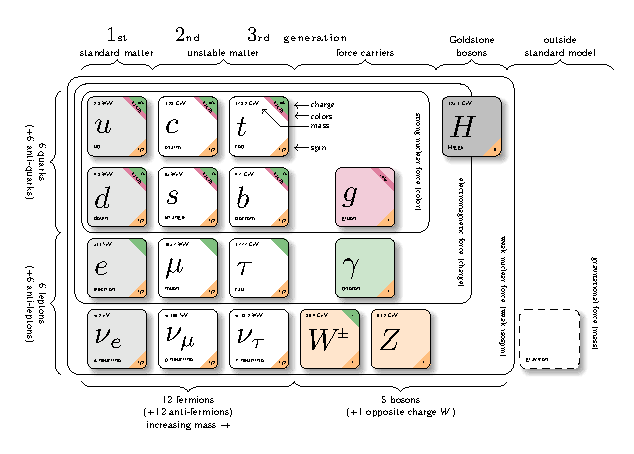
\includegraphics[width=0.8\textwidth]{fig/standard-model.pdf}
    %\caption{fig/standard-model.pdf}
    %\label{fig:fig-standard-model-pdf}
  \end{figure}
\end{frame}

\begin{frame}[fragile]{Supersymmetry}
  SUSY
\end{frame}

\begin{frame}[fragile]{Compressed Mass Spectrum}
  Compressed Mass Spectrum
\end{frame}

\begin{frame}[fragile]{Vector Boson Fusion Topology}
  VBF Topoloy
\end{frame}

\begin{frame}[fragile]{The LHC Collider}
  The largest and highest-energy particle collider in the world
  Housed in 
\end{frame}

\begin{frame}[fragile]{The CMS detector}
  CMS detector
\end{frame}

\begin{frame}[fragile]{Analysis Workflow}
  workflow
\end{frame}

\begin{frame}[fragile]{Event Selection}
  Event Selection
\end{frame}

\begin{frame}[fragile]{Background Estimation}
  Background Estimation
\end{frame}

\begin{frame}[fragile]{Statistical Inference}
  likelihood
\end{frame}

\begin{frame}[fragile]{Results}
  results
\end{frame}

\begin{frame}[fragile]{Conclusion}
  Conclusion
\end{frame}

\begin{frame}[fragile]{Outlook}
  outlook
\end{frame}
